\newpage
\section{Complexity Theory}

Asymptotic notations describe how algorithms perform as input size \((n)\) grows.

They help analyze:

\begin{itemize}
  
    \item \emph{Time Complexity}: How runtime grows.
  
    \item \emph{Space Complexity}: How memory usage grows.

\end{itemize}

\subsection{Definitions}

To clarify, all of these are sets of functions.

\subsubsection{\emph{Big O} \texorpdfstring{\((O)\)}{}} 
    
\begin{itemize}
    
    \item Upper Bound
    
    \item Describes the \emph{worst-case} growth rate.
    
    \item \(f(n) \in O(g(n))\) means \(\exists c, n_0\) such that \(\forall n > n_0, f(n) \leq c \cdot g(n)\). 
          In other words,  at some point our function \(f\) is always going to be less than \(g\).

\end{itemize}

\subsubsection{\emph{Omega} \texorpdfstring{\((\Omega)\)}{}} 
    
\begin{itemize}

    \item Lower Bound

    \item Describes the \emph{best-case} growth rate.

    \item \(f(n) \in \Omega(g(n))\) means \(\exists c, n_0\) such that \(\forall n > n_0, f(n) \geq c \cdot g(n)\). 
          In other words,  at some point our function \(f\) is always going to be greater than \(g\).

\end{itemize}

\subsubsection{\emph{Theta} \texorpdfstring{\((\Theta)\)}{}} 

\begin{itemize}

    \item Tight Bound

    \item Describes the \emph{average-case} or exact growth rate.

    \item \(f(n) \in \Theta(g(n))\) means \(f(n) \in O(g(n))\) and \(f(n) \in \Omega(g(n))\). 
          Means,  at some point our function \(f\) is always going be in between two bounds.

\end{itemize}

\textbf{Example I:}

\[
    f(n) = 4n^2 + 8n + 15 \in O(n^2)
\]

\begin{align*}
    f(n) &\le c n^2 \\
    4n^2 + 8n + 15 &\le c n^2 \\
    4n^2 + 8n + 15 &\le 4n^2 + 8n^2 + 15n^2  = 27n^2
\end{align*}

Thus, we have found a constant \(c = 27\), from which our function always less is then \(g = c n^2\). 
Therefore, \(f \int O(g)\).

\QED

\textbf{Example II:}

\[
    n^3 \notin O(n^2)
\]

Suppose the opposite, then 

\[
    n^3 \in O(n^2) \implies n^3 \le c n^2 \implies n \le c \forall n \ge \Naturals, c \in \Reals
\]

Choose \(n = \lceil n_0 + c + 1 \rceil\) which is a natural number.

\[
    \lceil n_0 + c + 1 \rceil \le c 
\]

This is a contradiction. Therefore, \(n^3 \notin O(n^2)\).

\QED

\subsection{Master's Theorem}

Help us find the time complexity of divide-and-conquer recurrences:  

\[
    T(n) = a T(\left\lceil\frac{b}{n}\right\rceil) + c(n^d)
\]

Where:

\begin{itemize}

    \item \(a \geq 1\) is the number of sub-problems

    \item \(b > 1\) is the factor by which the problem size shrinks

    \item \(c(n^d), d \ge 1\) is the cost of the work outside recursion (e.g., combining results)

\end{itemize}

Imagine a tree generated by each time we divide the problem until some point where solving it becomes 
trivial \(\Theta (1)\). This tree is going to have a depth of \(\log_b n\) which are the times 
we can divide the problem and a max width of \(n^{\log_b a}\) which is the number of leafs at the bottom.

\begin{center}
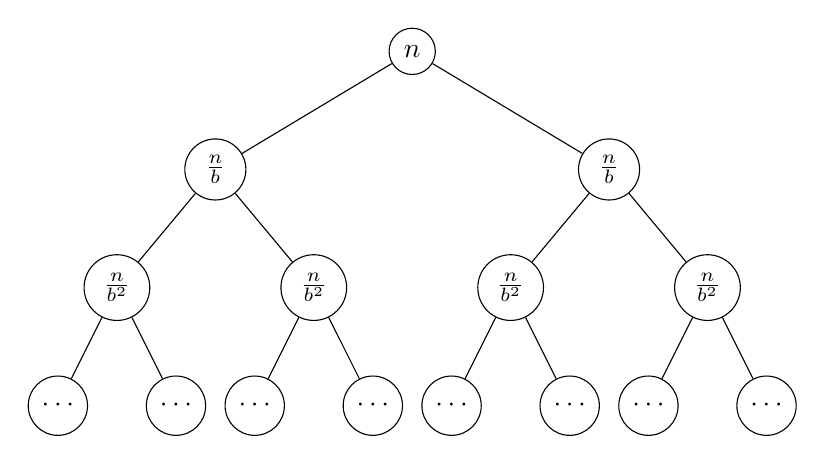
\begin{tikzpicture}
  [
    level distance=1.5cm,
    level 1/.style={sibling distance=5cm},
    level 2/.style={sibling distance=2.5cm},
    level 3/.style={sibling distance=1.5cm},
    every node/.style={circle, draw}
  ]
  \node {$n$}
    child {node {$\frac{n}{b}$}
      child {node {$\frac{n}{b^2}$}
        child {node {$\cdots$}}
        child {node {$\cdots$}}
      }
      child {node {$\frac{n}{b^2}$}
        child {node {$\cdots$}}
        child {node {$\cdots$}}
      }
    }
    child {node {$\frac{n}{b}$}
      child {node {$\frac{n}{b^2}$}
        child {node {$\cdots$}}
        child {node {$\cdots$}}
      }
      child {node {$\frac{n}{b^2}$}
        child {node {$\cdots$}}
        child {node {$\cdots$}}
      }
    };
\end{tikzpicture}
\end{center}

\[
    \text{Work at each level: } n, n, n, \ldots, n \Rightarrow \log n \text{ levels}
\]
\[
    \text{Total work: } n \log n
\]

Therefore, our total work is going to be 

\begin{align*}
    T(n) &= c(n) + a c(n/b) + a^2 c(b/n^2) + \cdots + \Theta(n^{log_b a})\\
         &=  \Theta(n^{log_b a}) + \sum_{j = 0}^{\log_b(n - 1)}a^j c (n/b^j)
\end{align*}

\subsubsection{Cases}

When looking at the tree generated by the divide-and-conquer we can get three cases:

\[
    T(n) \in
    \begin{cases}
        \text{The problem gets easier } &O(n^d) \text{ if } d > \log_b a \\
        \text{The hardness is evenly distributed } &O(n^d \log n) \text{ if } d = \log_b a \\
        \text{The problem get harder } &O(n^{\log_{b}a}) \text{ if } d < \log_b a \\
    \end{cases}
\]

\textbf{Example:}

\[
    T(n) = 4T (\frac{n}{2}) + c(n)
\]

Here \(a = 4\), \(b = 2\) and \(d = 1\). Since \(d < \log_b a\) \(1 < \log_2 4 = 2\) 

\[
    T(n) \in O(n^{log_b a} = O(n^2)
\]    


\subsection{How to Find Time Complexity}

\begin{enumerate}

    \item \textbf{Count Primitive Operations}

    \begin{itemize}

        \item Additions, multiplications, comparisons, etc.

    \end{itemize}

    \item \textbf{Identify Loops}

    \begin{itemize}

        \item Single loop \(\Rightarrow O(n)\)

        \item Nested loop \(\Rightarrow\) Multiply the complexities

    \end{itemize}

    \item \textbf{Check Recursive Patterns}

    \begin{itemize}

        \item Use recurrence relations (often solve with Master's Theorem)

    \end{itemize}

    \item \textbf{Ignore Constants}

    \begin{itemize}

        \item Drop lower-order terms and constants (e.g., \(O(n^2 + 3n + 5) \implies O(n^2)\))

    \end{itemize}

\end{enumerate}

\subsubsection{Examples}

\textbf{Example I: Simple Loop}

\begin{lstlisting}[language=Python]
for i in range(n):
    print(i)
\end{lstlisting}

\(\Rightarrow O(n)\)

\textbf{Example II: Nested Loop}

\begin{lstlisting}[language=Python]
for i in range(n):
    for j in range(n):
        print(i, j)
\end{lstlisting}

\(\Rightarrow O(n^2)\)

\subsection{Common Time Complexities}

\begin{center}
\begin{tabular}{|c|c|c|}
\hline
\textbf{Complexity} & \textbf{Name} & \textbf{Example Algorithms} \\
\hline
    \(O(1)\)       & Constant          & Array access \\
    \(O(\log n)\)  & Logarithmic       & Binary search \\
    \(O(n)\)       & Linear            & Linear search \\
    \(O(n \log n)\)& Linearithmic      & Merge Sort, Heap Sort \\
    \(O(n^2)\)     & Quadratic         & Bubble Sort, Selection Sort \\
    \(O(n^3)\)     & Cubic             & Naive matrix multiplication \\
    \(O(2^n)\)     & Exponential       & Recursive Fibonacci \\
    \(O(n!)\)      & Factorial         & Traveling Salesman (brute force) \\
    \hline
\end{tabular}
\end{center}
